% Options for packages loaded elsewhere
\PassOptionsToPackage{unicode}{hyperref}
\PassOptionsToPackage{hyphens}{url}
\PassOptionsToPackage{dvipsnames,svgnames,x11names}{xcolor}
%
\documentclass[
  letterpaper,
  DIV=11,
  numbers=noendperiod]{scrartcl}

\usepackage{amsmath,amssymb}
\usepackage{lmodern}
\usepackage{iftex}
\ifPDFTeX
  \usepackage[T1]{fontenc}
  \usepackage[utf8]{inputenc}
  \usepackage{textcomp} % provide euro and other symbols
\else % if luatex or xetex
  \usepackage{unicode-math}
  \defaultfontfeatures{Scale=MatchLowercase}
  \defaultfontfeatures[\rmfamily]{Ligatures=TeX,Scale=1}
\fi
% Use upquote if available, for straight quotes in verbatim environments
\IfFileExists{upquote.sty}{\usepackage{upquote}}{}
\IfFileExists{microtype.sty}{% use microtype if available
  \usepackage[]{microtype}
  \UseMicrotypeSet[protrusion]{basicmath} % disable protrusion for tt fonts
}{}
\makeatletter
\@ifundefined{KOMAClassName}{% if non-KOMA class
  \IfFileExists{parskip.sty}{%
    \usepackage{parskip}
  }{% else
    \setlength{\parindent}{0pt}
    \setlength{\parskip}{6pt plus 2pt minus 1pt}}
}{% if KOMA class
  \KOMAoptions{parskip=half}}
\makeatother
\usepackage{xcolor}
\setlength{\emergencystretch}{3em} % prevent overfull lines
\setcounter{secnumdepth}{5}
% Make \paragraph and \subparagraph free-standing
\ifx\paragraph\undefined\else
  \let\oldparagraph\paragraph
  \renewcommand{\paragraph}[1]{\oldparagraph{#1}\mbox{}}
\fi
\ifx\subparagraph\undefined\else
  \let\oldsubparagraph\subparagraph
  \renewcommand{\subparagraph}[1]{\oldsubparagraph{#1}\mbox{}}
\fi


\providecommand{\tightlist}{%
  \setlength{\itemsep}{0pt}\setlength{\parskip}{0pt}}\usepackage{longtable,booktabs,array}
\usepackage{calc} % for calculating minipage widths
% Correct order of tables after \paragraph or \subparagraph
\usepackage{etoolbox}
\makeatletter
\patchcmd\longtable{\par}{\if@noskipsec\mbox{}\fi\par}{}{}
\makeatother
% Allow footnotes in longtable head/foot
\IfFileExists{footnotehyper.sty}{\usepackage{footnotehyper}}{\usepackage{footnote}}
\makesavenoteenv{longtable}
\usepackage{graphicx}
\makeatletter
\def\maxwidth{\ifdim\Gin@nat@width>\linewidth\linewidth\else\Gin@nat@width\fi}
\def\maxheight{\ifdim\Gin@nat@height>\textheight\textheight\else\Gin@nat@height\fi}
\makeatother
% Scale images if necessary, so that they will not overflow the page
% margins by default, and it is still possible to overwrite the defaults
% using explicit options in \includegraphics[width, height, ...]{}
\setkeys{Gin}{width=\maxwidth,height=\maxheight,keepaspectratio}
% Set default figure placement to htbp
\makeatletter
\def\fps@figure{htbp}
\makeatother
\newlength{\cslhangindent}
\setlength{\cslhangindent}{1.5em}
\newlength{\csllabelwidth}
\setlength{\csllabelwidth}{3em}
\newlength{\cslentryspacingunit} % times entry-spacing
\setlength{\cslentryspacingunit}{\parskip}
\newenvironment{CSLReferences}[2] % #1 hanging-ident, #2 entry spacing
 {% don't indent paragraphs
  \setlength{\parindent}{0pt}
  % turn on hanging indent if param 1 is 1
  \ifodd #1
  \let\oldpar\par
  \def\par{\hangindent=\cslhangindent\oldpar}
  \fi
  % set entry spacing
  \setlength{\parskip}{#2\cslentryspacingunit}
 }%
 {}
\usepackage{calc}
\newcommand{\CSLBlock}[1]{#1\hfill\break}
\newcommand{\CSLLeftMargin}[1]{\parbox[t]{\csllabelwidth}{#1}}
\newcommand{\CSLRightInline}[1]{\parbox[t]{\linewidth - \csllabelwidth}{#1}\break}
\newcommand{\CSLIndent}[1]{\hspace{\cslhangindent}#1}

\usepackage{booktabs}
\usepackage{longtable}
\usepackage{array}
\usepackage{multirow}
\usepackage{wrapfig}
\usepackage{float}
\usepackage{colortbl}
\usepackage{pdflscape}
\usepackage{tabu}
\usepackage{threeparttable}
\usepackage{threeparttablex}
\usepackage[normalem]{ulem}
\usepackage{makecell}
\usepackage{xcolor}
\KOMAoption{captions}{tableheading}
\makeatletter
\makeatother
\makeatletter
\makeatother
\makeatletter
\@ifpackageloaded{caption}{}{\usepackage{caption}}
\AtBeginDocument{%
\ifdefined\contentsname
  \renewcommand*\contentsname{Table of contents}
\else
  \newcommand\contentsname{Table of contents}
\fi
\ifdefined\listfigurename
  \renewcommand*\listfigurename{List of Figures}
\else
  \newcommand\listfigurename{List of Figures}
\fi
\ifdefined\listtablename
  \renewcommand*\listtablename{List of Tables}
\else
  \newcommand\listtablename{List of Tables}
\fi
\ifdefined\figurename
  \renewcommand*\figurename{Figure}
\else
  \newcommand\figurename{Figure}
\fi
\ifdefined\tablename
  \renewcommand*\tablename{Table}
\else
  \newcommand\tablename{Table}
\fi
}
\@ifpackageloaded{float}{}{\usepackage{float}}
\floatstyle{ruled}
\@ifundefined{c@chapter}{\newfloat{codelisting}{h}{lop}}{\newfloat{codelisting}{h}{lop}[chapter]}
\floatname{codelisting}{Listing}
\newcommand*\listoflistings{\listof{codelisting}{List of Listings}}
\makeatother
\makeatletter
\@ifpackageloaded{caption}{}{\usepackage{caption}}
\@ifpackageloaded{subcaption}{}{\usepackage{subcaption}}
\makeatother
\makeatletter
\@ifpackageloaded{tcolorbox}{}{\usepackage[many]{tcolorbox}}
\makeatother
\makeatletter
\@ifundefined{shadecolor}{\definecolor{shadecolor}{rgb}{.97, .97, .97}}
\makeatother
\makeatletter
\makeatother
\ifLuaTeX
  \usepackage{selnolig}  % disable illegal ligatures
\fi
\IfFileExists{bookmark.sty}{\usepackage{bookmark}}{\usepackage{hyperref}}
\IfFileExists{xurl.sty}{\usepackage{xurl}}{} % add URL line breaks if available
\urlstyle{same} % disable monospaced font for URLs
\hypersetup{
  pdftitle={Colorism and Cosmetics: Investigating Limited Shade Ranges in the Beauty Industry in Japan and India},
  pdfauthor={Laura Lee-Chu},
  colorlinks=true,
  linkcolor={blue},
  filecolor={Maroon},
  citecolor={Blue},
  urlcolor={Blue},
  pdfcreator={LaTeX via pandoc}}

\title{Colorism and Cosmetics: Investigating Limited Shade Ranges in the
Beauty Industry in Japan and India\thanks{Code and data supporting this
analysis is available at:}}
\author{Laura Lee-Chu}
\date{April 21, 2023}

\begin{document}
\maketitle
\begin{abstract}
This research paper explores the issue of colorism in the context of the
beauty industry in Japan and India. Drawing on data from an article
published by The Pudding, the paper focuses on the association between
the lightness and saturation of foundation shades provided by leading
makeup brands in India and Japan. The findings reveal a preference for
lighter shades in international brands, whereas domestic brands offer a
broader spectrum of shades with warmer undertones. The study uncovers a
negative correlation between the saturation and lightness of foundation
shades, with Japanese foundation shades being paler and having an ashier
tone, and Indian foundation shades being substantially lighter than the
natural skin tone. The scarcity of foundation shades for individuals
with darker skin tones can lead to their marginalization and exclusion,
perpetuating the issue of colorism in the beauty industry.
\end{abstract}
\ifdefined\Shaded\renewenvironment{Shaded}{\begin{tcolorbox}[sharp corners, interior hidden, boxrule=0pt, enhanced, frame hidden, breakable, borderline west={3pt}{0pt}{shadecolor}]}{\end{tcolorbox}}\fi

\renewcommand*\contentsname{Table of contents}
{
\hypersetup{linkcolor=}
\setcounter{tocdepth}{3}
\tableofcontents
}
\newpage

\hypertarget{introduction}{%
\section{Introduction}\label{introduction}}

The issue of colorism has been a persistent and pervasive concern across
the world. In societies where attractiveness is highly valued, women
often rely on makeup to enhance their appearance, with companies
capitalizing on these insecurities to promote their products. With the
growing popularity of makeup brands, the beauty industry has perpetuated
and exacerbated colorism, particularly in Japan and India, which are
among the largest beauty markets in Asia.

The roots of colorism in Japan and India have historical and cultural
origins that have contributed to the perpetuation of this issue in
modern society. In Japan, the association of fair skin with beauty and
status can be traced back to its aristocracy, who were able to avoid
outdoor labour and maintain a pale complexion (Phoenix 2014). This idea
became ingrained in Japanese society and is reinforced through media,
advertising, and popular culture. The influence of Western beauty
standards, introduced through the influx of mass media from the United
States after World War II, has also contributed to the shift towards
lighter skin tones in Japan (Phoenix 2014).

Similarly, in India, the issue of colorism has been exacerbated by the
history of colonialism, with the British favouring Indians with lighter
skin for government jobs. This discrimination based on skin colour has
persisted in Indian society, with fair skin being equated with higher
social status and dark skin being associated with lower status
(Jayawardene 2016). The impacts of colorism in India are widespread,
affecting social mobility, education, employment, and marriage.

In addition to the negative impact on individuals, colorism also has
wider societal consequences. Individuals with darker skin tones face
exclusion and marginalization, as well as limited access to products and
services, leading to unequal opportunities in various aspects of life
(Phoenix 2014). The globalization of beauty standards has further
compounded the issue, with Western ideals of beauty being prioritized
and perpetuated by the beauty industry.

To better understand the issue of colorism in Japan and India, the
present study draws on data from an article published by The Pudding, a
digital publisher specializing in data journalism. The original article
examined the lack of diversity in makeup shades offered by major
cosmetic brands (Jason Li 2018). However, the current study will focus
specifically on the context of Asia and the role of colorism in
perpetuating limited shade ranges, with a particular focus on Japan and
India.

This paper examines the association between the lightness and saturation
of foundation shades provided by leading makeup brands in India and
Japan. The findings revealed that international brands exhibit a
preference for lighter shades, whereas domestic brands offer a broader
spectrum of shades with warmer undertones. A linear regression model was
employed, and a noteworthy negative correlation was discovered between
the saturation and lightness of foundation shades. Specifically, as
saturation rises, the expected lightness of the foundation shade
diminishes. The study further unveiled that, on average, Japanese
foundation shades are paler and have an ashier tone, whereas Indian
foundation shades are substantially lighter than the natural skin tone.
This scarcity of foundation shades for individuals with darker skin
tones can lead to their marginalization and exclusion.

\newpage

\hypertarget{data}{%
\section{Data}\label{data}}

This paper was produced using the R statistical programming language (R
Core Team 2022). here was used to reference file locations (Müller
2020). The data was examined and cleaned using the packages janitor
(Firke 2021), dplyr (Wickham et al. 2023), and tidyverse (Wickham et al.
2019). Tables were made knitr (Xie 2023) and broom (0.7.11 2021), and
formatted with kableExtra (Zhu 2021). ggplot2 (Wickham 2016) was used to
plot and scale the graphs.

\hypertarget{the-dataset}{%
\subsection{The Dataset}\label{the-dataset}}

The dataset was specifically curated for application in The Pudding
essay entitled ``Beauty Brawl,'' which was published in June of 2018
(Jason Li 2018). The data was obtained through a systematic process that
involved identifying prominent beauty brands in the United States,
Nigeria, India, and Japan, as well as consulting various sources that
verified their status as best-selling products within their respective
domestic markets. The research team accessed each of the brand's
official websites in May of 2018 and isolated their liquid foundation
collection that possessed the most extensive variety of available
shades. For each colour swatch displayed for the product, the
corresponding hex colour values were recorded. Subsequently, Adobe
Photoshop was utilized to extract the lightness value of each colour
using the CIE Lab colour model.

To further classify the sampled products, two additional columns were
incorporated into the dataset. These columns included ``Brand,'' which
provided the complete written title of the brand responsible for
producing the specific foundation shade, and ``Product,'' which listed
the full name of the sampled foundation product. It should be noted that
for certain brands, this foundation line represented their sole range of
liquid foundation, while for others, it constituted the product line
containing the largest quantity of available shades.

Moreover, it is worth noting that each product within the dataset is
exclusively assigned to a single group. In the dataset, a total of seven
distinct groups were employed for classification:

\begin{itemize}
\tightlist
\item
  0: Fenty Beauty's PRO FILT'R Foundation Only
\item
  1: Make Up For Ever's Ultra HD Foundation Only
\item
  2: US Best Sellers
\item
  3: BIPOC-recommended Brands with BIPOC Founders
\item
  4: BIPOC-recommended Brands with White Founders
\item
  5: Nigerian Best Sellers
\item
  6: Japanese Best Sellers
\item
  7: Indian Best Sellers
\end{itemize}

The dataset included information on the hexadecimal colour code (hex),
hue (angle on the colour wheel), saturation (degree of colour/chroma),
and brightness (also known as value, which measures the lightness or
darkness halfway point) values of the foundation shades. The lightness
(the relative degree of black or white) values were derived using the
CIE Lab colour model, which is predicated on the human perception of
colour. The numerical values in the CIE Lab model describe the full
spectrum of colours that are visible to individuals with normal vision.
As the CIE Lab model represents how a colour appears rather than
specifying the quantity of a particular colourant required for a
particular device (such as a digital camera, monitor, or desktop
printer) to generate colours, it is regarded as a device-independent
colour model. To ensure reliable and consistent colour transformation
from one colour space to another, colour management systems use the CIE
Lab model as a reference point (Adobe 2022).

One of the limitations of the dataset used in this study is that it only
covers data from 2018. Since then, various social movements have taken
place around the world that may have influenced the range of foundation
shades offered by makeup brands. Furthermore, the hex codes used in the
dataset do not provide any meaningful information unless visually
modelled. However, due to the large number of values and their lack of
proper notation, the process of visual modelling is extremely
time-consuming. Unfortunately, no other datasets with similar or related
content were available for use in this study.

This study primarily employs lightness values (L*) to quantify the
degree of lightness or darkness in foundation shades and Saturation to
evaluate foundation undertone shades. The lightness values are
represented on a scale of 0-100, with 100 being the highest value,
indicating the lightest shade. Saturation is measured as the amount of
gray present in a colour, using a decimal value between 0 and 1. The
degree of saturation is directly proportional to the vividness and
intensity of the colour. Conversely, a low level of saturation implies a
colour that is closer to pure gray on the grayscale.

\hypertarget{data-cleaning}{%
\subsection{Data Cleaning}\label{data-cleaning}}

To narrow the scope of the study to Asia, the focus was shifted to only
include India and Japan, leading to the filtering of the dataset to only
retain these two groups. The data was further refined by isolating
brand, lightness, and saturation values, with the lightness values being
grouped into ranges of 10. Subsequently, each makeup brand was
researched individually to classify them as either domestic or
international, to assess any potential differences in shade ranges
between these two categories. While the dataset contained information on
multiple products from a single brand, this study aims to explore the
wider implications of the shade ranges offered within each country.

\begin{table}

\caption{Table 1: Total number of products by lightness range in India & Japan}
\centering
\begin{tabular}[t]{l|r|r|r|r|r|r}
\hline
\multicolumn{1}{c|}{ } & \multicolumn{6}{c}{Lightness Range} \\
\cline{2-7}
Country & 20 - 30 & 50-60 & 60-70 & 70-80 & 80-90 & Total\\
\hline
India & 1 & 3 & 14 & 23 & 16 & 57\\
\hline
Japan & 0 & 3 & 12 & 32 & 27 & 74\\
\hline
\end{tabular}
\end{table}

The dataset comprises 9 distinct brands for India and 8 for Japan. Table
2 indicates that Japan features a greater number of shades compared to
India. Nevertheless, both countries exhibit a similar pattern of maximum
product offerings in the 70-80 shade range, followed by the 80-90 range
as the second-highest, and subsequently the 60-70 and 50-60 ranges.
Notably, only one product belonging to India is classified in the 20-30
shade range, while Japan has none. Furthermore, the table demonstrates
that Japan and India share a comparable distribution of lightness among
their product ranges.

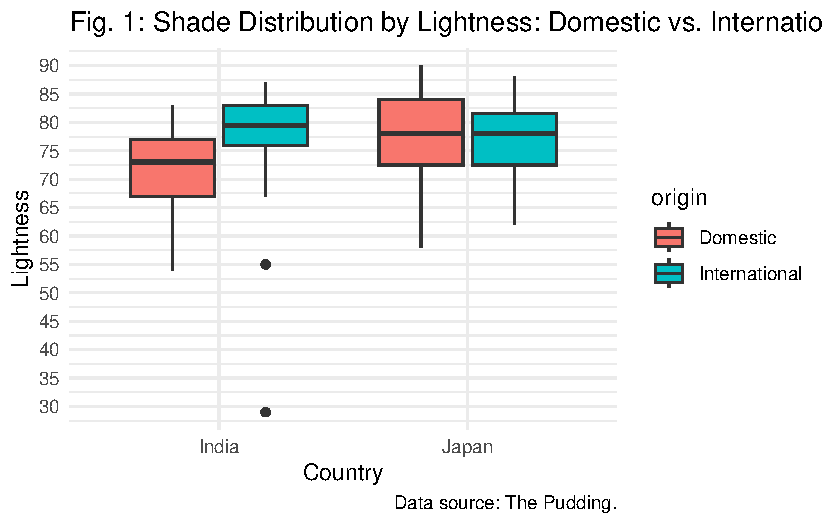
\includegraphics{paper_files/figure-pdf/unnamed-chunk-3-1.pdf}

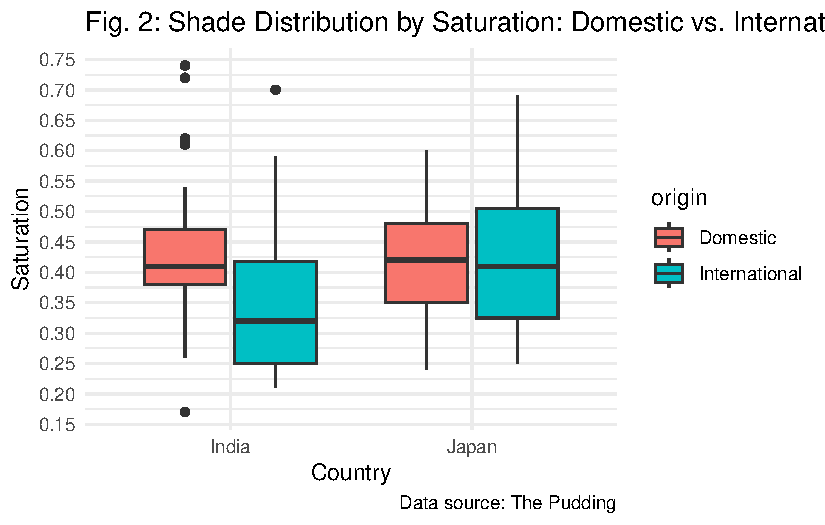
\includegraphics{paper_files/figure-pdf/unnamed-chunk-4-1.pdf}

As depicted in Figure 1, the analysis of the Indian market reveals that
international brands exhibit a noticeable bias towards lighter shades
with a relatively smaller interquartile range, higher median, and
maximum. In contrast, domestic brands demonstrate a larger interquartile
range and lower median. However, it is noteworthy that an international
brand in India has an outlier with a considerably lower lightness value
in the 20-30 range. In contrast, the Japanese market displays a
different pattern where both international and domestic brands have the
same median, but domestic brands present a wider range. Furthermore, in
contrast to the Indian market, Japanese domestic brands feature not only
darker shades but also a greater variety of lighter shades.

Nevertheless, a contrasting trend emerges when considering the
undertones of foundation products. Figure 2 illustrates the saturation
distribution between international and domestic brands, revealing that
in both the Indian and Japanese markets, international brands exhibit a
wider range of saturation compared to their domestic counterparts. In
India, domestic brands demonstrate a significantly higher median
saturation, implying a warmer tone, with a multitude of outliers
situated at the upper end of the saturation scale. Conversely,
international brands feature a significantly lower median saturation,
indicating a cooler or ashy tone. In Japan, both domestic and
international brands have a similar median saturation, with domestic
brands marginally higher. However, international brands have a
significantly higher maximum saturation, indicating warm undertones and
domestic brands feature a lower minimum saturation.

\newpage

\hypertarget{model}{%
\section{Model}\label{model}}

Given the similarity in lightness observed in foundation shades across
both countries, it was of interest to investigate if any differences in
saturation existed. This investigation was motivated by the fact that
the local population in each country has unique undertones. Before
conducting the analysis, several tests were conducted to verify that the
model assumptions (See Appendix A), including linearity, normality, and
homoscedasticity of residuals, were satisfied, thereby ensuring that the
model was well-suited for the data at hand.

The null hypothesis: there is no significant linear relationship between
the lightness of foundation shades and the saturation of undertones.

The alternative hypothesis: there is a significant linear relationship
between the lightness of foundation shades and the saturation of
undertones.

A linear regression analysis can be conducted to test this hypothesis
and to determine whether a statistically significant relationship exists
between the variables. A low p-value for the regression coefficient for
saturation would provide evidence against the null hypothesis,
indicating that changes in saturation do result in a meaningful
variation in lightness across foundation shades. On the other hand, if
the p-value is high, this would suggest that there is not enough
evidence to reject the null hypothesis, and there may be no significant
linear relationship between the variables. Ultimately, the results of
the analysis will inform whether the null hypothesis can be rejected or
not. The mathematical equation for the linear regression model can be
written as:

\[L = \beta_0 + \beta_1S + \epsilon\]

Where:

\begin{itemize}
\tightlist
\item
  \(L\) represents the dependent variable, which is the overall
  lightness of the foundation shade
\item
  \(S\) represents the independent variable, which is the saturation of
  the foundation shade
\item
  \(\beta_0\) represents the intercept of the regression line, which is
  the predicted value of \(L\) when \(S\) is equal to zero
\item
  \(\beta_1\) represents the slope of the regression line, which is the
  change in \(L\) for a one-unit increase in \(S\)
\item
  \(\epsilon\) represents the random error term, which accounts for
  variability in \(L\) that is not explained by the relationship with
  \(S\)
\end{itemize}

The aim of linear regression is to estimate the values of \(\beta_0\)
and \(\beta_1\) that minimize the sum of squared errors between the
predicted and actual values of lightness (\(L\)) for the given values of
saturation (\(S\)) in the dataset. By minimizing this sum of squared
errors, the linear regression model can produce the best-fit line to
describe the linear relationship between the two variables, allowing for
the estimation of \(L\) values based on known \(S\) values.

In this project, the lightness variable (\(L\)) is measured on a scale
of 0 to 100, while the saturation variable (\(S\)) is measured on a
scale of 0 to 1. Therefore, the slope coefficient \(\beta_1\) in the
linear regression model would represent the change in lightness (\(L\))
for a one-unit increase in saturation (\(S\)), where a one-unit increase
in \(S\) corresponds to an increase of 1/100 in the saturation of the
foundation shade. The intercept \(\beta_0\) in the model would represent
the expected value of \(L\) when \(S\) is equal to zero, which in this
case would correspond to the lightness value for a completely
desaturated foundation shade.

\newpage

\hypertarget{results}{%
\section{Results}\label{results}}

\begin{table}

\caption{Table 2: Linear Regression Model Summary}
\centering
\begin{tabular}[t]{l|r|r|r|r}
\hline
term & estimate & std.error & statistic & p.value\\
\hline
(Intercept) & 100.31483 & 1.962350 & 51.11973 & 0\\
\hline
S & -60.59635 & 4.666169 & -12.98632 & 0\\
\hline
\end{tabular}
\end{table}

This study employed a linear regression model to investigate the
association between the lightness (L) and saturation (S) of foundation
shades offered by popular makeup brands in Japan and India. As presented
in Table 2, the model yielded an estimated intercept of 100.31483,
indicating that the expected lightness of foundation shades when
saturation is zero is 100.31483. The model also revealed a statistically
significant negative regression coefficient of -60.59635 for saturation
(t = -12.98632, p \textless{} .001), indicating a significant negative
linear relationship between saturation and lightness of foundation
shades.

These findings suggest that as the saturation of a foundation shade
increases, the predicted lightness of that shade decreases by
approximately 60.59635 units, holding all other variables constant. This
indicates that the foundation shades with higher saturation tend to be
darker, while those with lower saturation tend to be lighter.
Furthermore, the obtained intercept value of 100.31483 implies that the
range of foundation shades provided by the examined brands is generally
on the lighter end in both Japan and India.

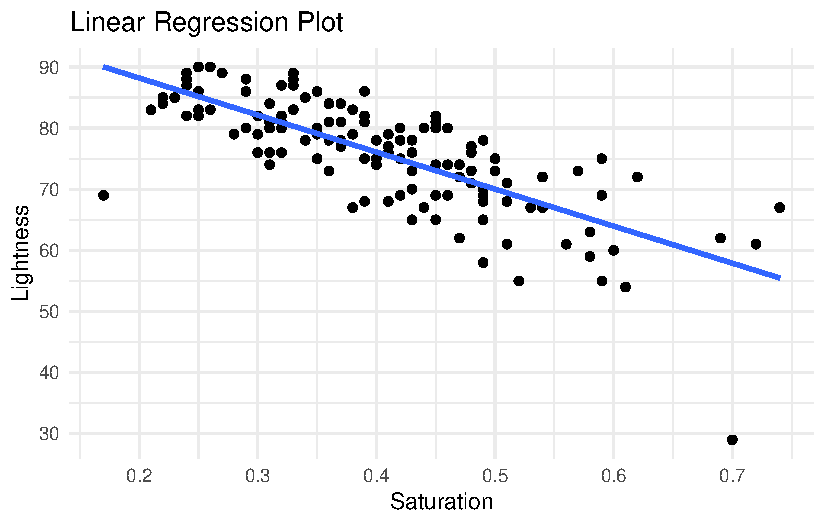
\includegraphics{paper_files/figure-pdf/unnamed-chunk-6-1.pdf}

Figure 3 illustrates this relationship between saturation and lightness,
where a scatterplot of the data points with saturation on the x-axis and
lightness on the y-axis shows a clear downward slope. The fitted
regression line represents the overall trend of the data, with the slope
indicating that as saturation increases, the predicted lightness of the
foundation shade decreases. It is worth noting that the intercept value
of 100.31483 is not a meaningful value in this context since a
foundation shade cannot have zero saturation.

\newpage

\hypertarget{discussion}{%
\section{Discussion}\label{discussion}}

In order to provide a more detailed exposition of the results obtained
from the model, an additional investigation was conducted on the
relationship between lightness and saturation for both international and
domestic brands within each country.

\hypertarget{japanese-foundation-shades-tend-to-be-lighter-and-ashier-on-average.}{%
\subsection{Japanese foundation shades tend to be lighter and ashier on
average.}\label{japanese-foundation-shades-tend-to-be-lighter-and-ashier-on-average.}}

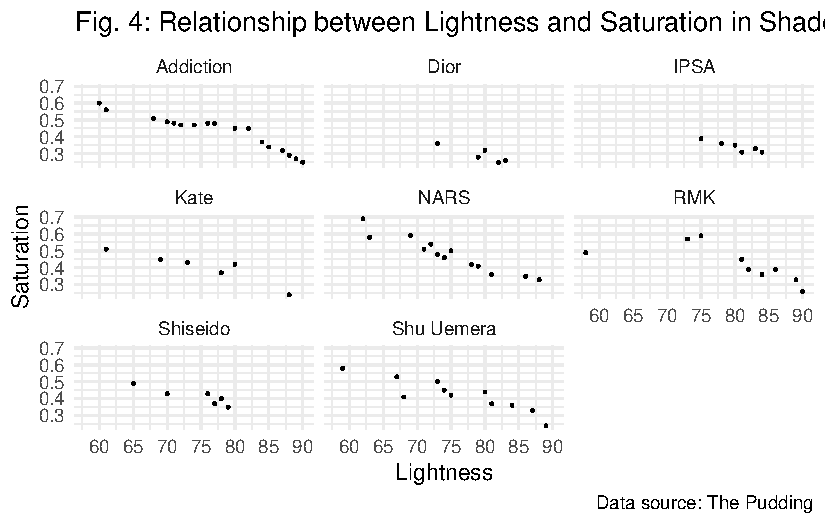
\includegraphics{paper_files/figure-pdf/unnamed-chunk-7-1.pdf}

In Japan, a negative linear relationship between the saturation and
lightness of foundation shades is observed, as depicted in Figure 4. The
data indicates that as the lightness of foundation shades increases,
their saturation decreases, suggesting that lighter foundations tend to
appear ashier or cooler-toned than their darker counterparts. According
to a study conducted by L'Oréal, East Asian women have a skin tone range
of 55-75 in lightness with warmer tones (Stephanie Nouveau 2014). The
brands closest to the regression line seen in Figure 3 with the widest
range in lightness and saturation are Addiction, NARS, and Shu Uemera,
as demonstrated in Figure 4.

When comparing domestic and international brand offerings, it is
noteworthy that Japanese brands, including Addiction, Kate, Shu Uemura,
and RMK, offer shades in the 85-90 lightness range, which is
significantly lighter than the skin tone range. NARS, originally a
foreign brand but now a subsidiary of Shiseido, offers a wider range of
shades in both saturation and lightness in contrast with Shiseido.
Conversely, although Shu Uemera, a Japanese brand, was acquired by
L'Oréal, it still maintains a wide distribution. In contrast, the
international luxury brand Dior only offers cool-toned shades within the
lighter end of the skin tone range.

The data suggest that foundation offerings in Japan tend to skew toward
the fairer end of the skin tone range or significantly lighter. While
there are options available for Japanese consumers to find foundation
within their skin-tone range, the average foundation shade is lighter
and ashier, reflecting a preference for fairer skin, and reinforcing the
notion that lighter skin is more desirable. This reinforces the societal
pressure to conform to certain beauty standards and can exacerbate
colorism by perpetuating the notion that lighter skin is superior to
darker skin tones (Phoenix 2014). The negative correlation between
saturation and lightness observed in the data also implies that
consumers with warmer undertones may encounter difficulties in finding
foundation shades that strike the appropriate balance between warmth and
lightness. Specifically, they may find that foundation shades with warm
undertones are excessively dark, while those with cooler undertones are
excessively light. This highlights the necessity for makeup brands to
provide a diverse range of foundation shades that cater to a variety of
undertones and levels of saturation.

\newpage

\hypertarget{indian-foundation-shades-are-significantly-lighter-than-the-natural-skin-tone.}{%
\subsection{Indian foundation shades are significantly lighter than the
natural skin
tone.}\label{indian-foundation-shades-are-significantly-lighter-than-the-natural-skin-tone.}}

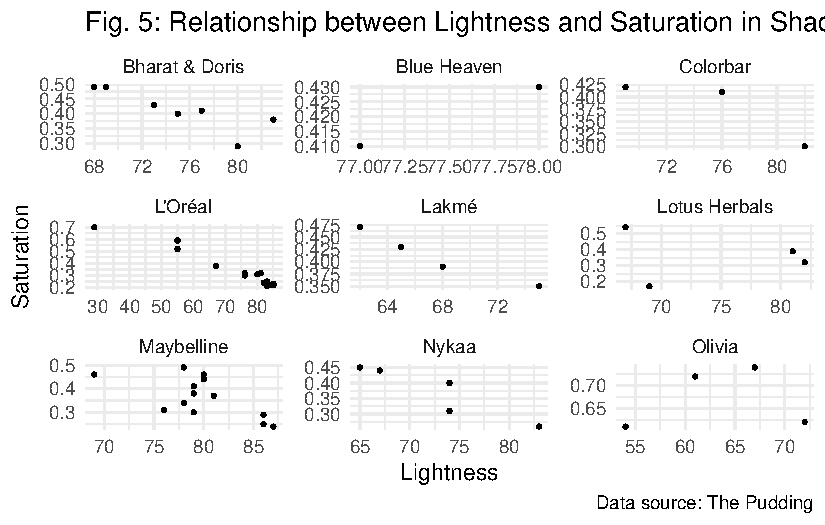
\includegraphics{paper_files/figure-pdf/unnamed-chunk-8-1.pdf}

Figure 5 presents a noteworthy disparity in the distribution of
foundation shades across various brands concerning their lightness and
saturation attributes. Specifically, it appears that domestic brands in
India offer fewer foundation shades compared to international brands
like L'Oréal and Maybelline. However, despite Indian skin tones falling
within a lightness range of 30-65 and exhibiting warm-toned features,
the majority of foundation shades offered by international brands are
noticeably situated in the 70-85 lightness range (Stephanie Nouveau
2014). This observation suggests that international brands tend to
prioritize whiteness more than local brands.

Nevertheless, it is important to note that L'Oréal is the only
international brand that offers a shade of around 30 with higher
saturation. In contrast, the darkest shade provided by a domestic brand
is approximately 50, offered by Olivia, which presents all of their
products with a warmer tone in contrast to other brands. Furthermore,
excluding Lakmé and Olivia, all other domestic brands commence their
shade range beyond the maximum limit of the skin tone range. This
indicates that Indian consumers tend to purchase foundation shades that
are significantly lighter and cooler than their natural skin tone.

The data highlights the tendency of international brands to prioritize
whiteness, and the scarcity of shades available for consumers with
darker skin tones, which may contribute to the perpetuation of colorism.
Furthermore, the limited availability of foundation shades for those
with darker skin tones can result in the exclusion and marginalization
of individuals with such skin tones.

\newpage

\hypertarget{weaknesses-next-steps}{%
\subsection{Weaknesses \& Next Steps}\label{weaknesses-next-steps}}

The findings of this study indicate that foundation shades offered in
both Indian and Japanese markets tend to lean towards lighter shades.
However, one of the limitations of this study is the lack of a visual
representation of the shades and colours of the data points, which makes
it more difficult to visualize the relationship between saturation,
lightness, and the range of foundation shades offered by makeup brands.
Additionally, since there was no comparable dataset available for the
skin tone study, it is challenging to gauge the extent to which the
foundation offerings are lighter than the natural skin tone range. These
limitations may impact the accuracy and comprehensibility of the
findings of this study.

The roots of colorism in Japan and India can be traced back to its
cultural and historical context, and it has significant impacts on
individuals and society, perpetuating discrimination and exclusion. The
data suggests that there is room for improvement in the range of
foundation shades offered by makeup brands in both Japan and India. By
offering a more diverse range of shades that cater to a variety of
undertones and levels of saturation, makeup brands can better serve the
needs of their consumers and ensure that everyone has access to makeup
products that match their skin tone. Addressing this issue requires a
collective effort from all stakeholders, including policymakers, the
beauty industry, and society as a whole, to promote a more inclusive and
accepting culture that celebrates diversity and rejects discriminatory
beauty standards.

\newpage

\hypertarget{appendix}{%
\section{Appendix}\label{appendix}}

\hypertarget{model-testing}{%
\subsection{Model Testing}\label{model-testing}}

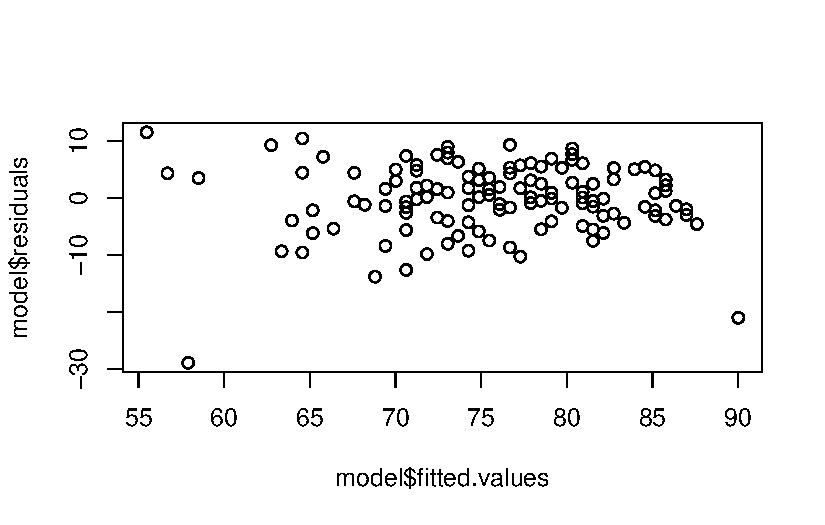
\includegraphics{paper_files/figure-pdf/unnamed-chunk-9-1.pdf}

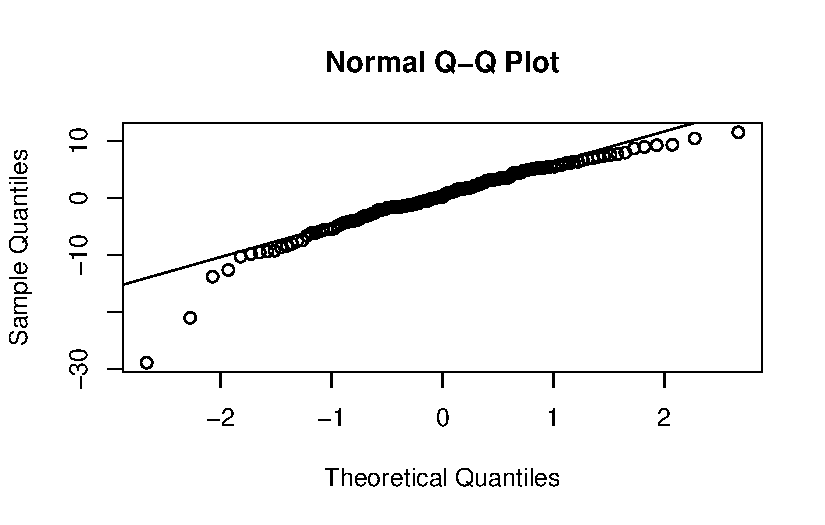
\includegraphics{paper_files/figure-pdf/unnamed-chunk-9-2.pdf}

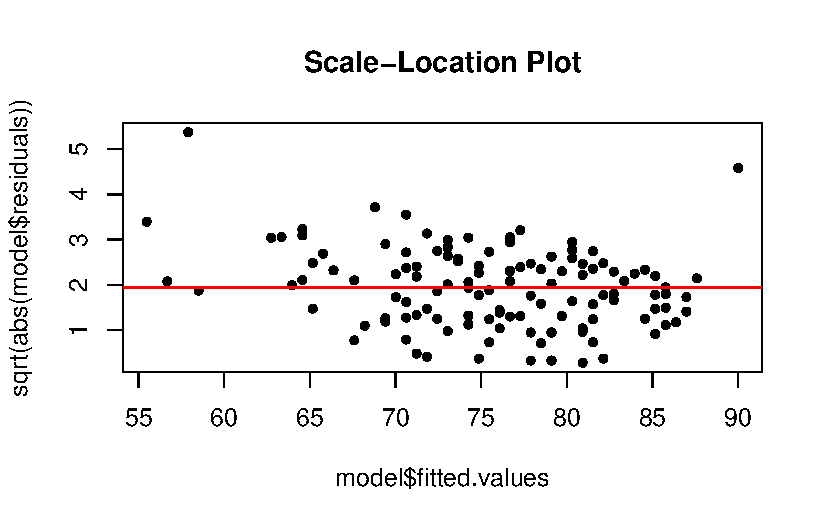
\includegraphics{paper_files/figure-pdf/unnamed-chunk-9-3.pdf}

\newpage

\hypertarget{references}{%
\section{References}\label{references}}

\hypertarget{refs}{}
\begin{CSLReferences}{1}{0}
\leavevmode\vadjust pre{\hypertarget{ref-broom}{}}%
0.7.11, R package version. 2021. \emph{Broom: Convert Statistical
Objects into Tidy Tibbles}.

\leavevmode\vadjust pre{\hypertarget{ref-adobe}{}}%
Adobe. 2022. \emph{Lab Color Mode}.

\leavevmode\vadjust pre{\hypertarget{ref-janitor}{}}%
Firke, Sam. 2021. \emph{Janitor: Simple Tools for Examining and Cleaning
Dirty Data}. \url{https://github.com/sfirke/janitor}.

\leavevmode\vadjust pre{\hypertarget{ref-pudding}{}}%
Jason Li, Divya Manian, Amber Thomas. 2018. \emph{BEAUTY BRAWL}.

\leavevmode\vadjust pre{\hypertarget{ref-india}{}}%
Jayawardene, Sureshi M. 2016. \emph{Racialized Casteism: Exposing the
Relationship Between Race, Caste, and Colorism Through the Experiences
of Africana People in India and Sri Lanka}.

\leavevmode\vadjust pre{\hypertarget{ref-here}{}}%
Müller, Kirill. 2020. \emph{Here: A Simpler Way to Find Your Files}.

\leavevmode\vadjust pre{\hypertarget{ref-japan}{}}%
Phoenix, Aisha. 2014. \emph{Colourism and the Politics of Beauty}.

\leavevmode\vadjust pre{\hypertarget{ref-citeR}{}}%
R Core Team. 2022. \emph{R: A Language and Environment for Statistical
Computing}. Vienna, Austria: R Foundation for Statistical Computing.
\url{https://www.R-project.org/}.

\leavevmode\vadjust pre{\hypertarget{ref-loreal}{}}%
Stephanie Nouveau, Frederic Flament. 2014. \emph{Skin Color Types and
Indian Skin Characteristics}.

\leavevmode\vadjust pre{\hypertarget{ref-ggplot2}{}}%
Wickham, Hadley. 2016. \emph{Ggplot2: Elegant Graphics for Data
Analysis}. Springer-Verlag New York.
\url{https://ggplot2.tidyverse.org}.

\leavevmode\vadjust pre{\hypertarget{ref-tidyverse}{}}%
Wickham, Hadley, Mara Averick, Jennifer Bryan, Winston Chang, Lucy
D'Agostino McGowan, Romain François, Garrett Grolemund, et al. 2019.
{``Welcome to the {tidyverse}.''} \emph{Journal of Open Source Software}
4 (43): 1686. \url{https://doi.org/10.21105/joss.01686}.

\leavevmode\vadjust pre{\hypertarget{ref-dplyr}{}}%
Wickham, Hadley, Romain François, Lionel Henry, Kirill Müller, and Davis
Vaughan. 2023. \emph{Dplyr: A Grammar of Data Manipulation}.

\leavevmode\vadjust pre{\hypertarget{ref-knitr}{}}%
Xie, Yihui. 2023. \emph{Knitr: A General-Purpose Package for Dynamic
Report Generation in r}. \url{https://yihui.org/knitr/}.

\leavevmode\vadjust pre{\hypertarget{ref-kableExtra}{}}%
Zhu, Hao. 2021. \emph{kableExtra: Construct Complex Table with 'Kable'
and Pipe Syntax}.

\end{CSLReferences}



\end{document}
